\documentclass{article}

\usepackage[%
    left=0.5in,%
    right=0.5in,%
    top=0.5in,%
    bottom=0.5in,%
]{geometry}%
\usepackage{minitoc}
\usepackage{multicol}
\usepackage{graphicx}
\usepackage{fixltx2e}
\usepackage{listings}
\usepackage{color}
\usepackage{hyperref}
    \hypersetup{ colorlinks = true, linkcolor = blue }
\usepackage{blindtext}
\definecolor{lightgray}{gray}{0.9}
\graphicspath{ {./} }

\newcommand{\inlinecode}[2]{\colorbox{lightgray}{\lstinline
[language=#1]$#2$}}
\newcommand{\worddef}[1]{\hyperref[sec:reference]{\textit{#1}}}

\begin{document}

\tableofcontents

\newpage

\section{Limitations of simple reactive architecture}
no representation of the environment means
\begin{itemize}
  \item its knowledge of the world is limited by the \textbf{range of its sensors }
  \item it’s unable to count (as opposed to recognise number)
  \item it’s unable to recover from actions which fail silently – and many others
\end{itemize}

\begin{multicols}{2}

\section{Modelling reactive behaviours}
\begin{center}
  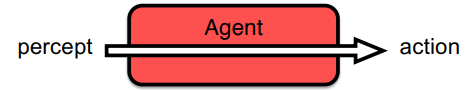
\includegraphics[scale=0.5]{reactive_agent.png}
\end{center}

\begin{itemize}
  \item we can model reactive behaviours as condition-action rules 
  \item if the condition matches the agent’s precepts, it triggers an action \texttt{if percept then action }
  \item a simple reactive agent maintains no internal representation of the state of the world, whether the rule has been fired before etc.
\end{itemize}


\section{Reactive architectures with state}

\begin{center}
  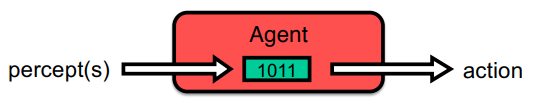
\includegraphics[scale=0.5]{reactive_state_agent.png}
\end{center}

\begin{itemize}
  \item some rules match against an internal representation of aspects of the environment 
  \item representations can be built using simple \textbf{percept-driven rules} (internal actions) which record simple ‘beliefs’ about the state of the world
\end{itemize}

\end{multicols}

\section{State}

\begin{itemize}
  \item we have simply taken a condition-action rule which matched against a percept and generated an action and split it in two, with a mediating internal representation 
  \item needs extra machinery to store the state 
  \item requires at least \textbf{two computation steps} to choose an action rather than one
\end{itemize}

\subsection{Actions which modify the internal state}

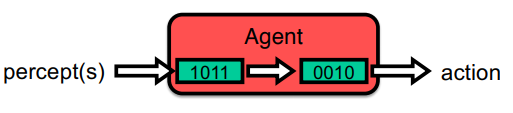
\includegraphics[scale=0.5]{reactive_state_agent_modify.png}

\begin{itemize}
  \item we can extend this to rules
  \begin{itemize}
    \item whose conditions match against the agent’s internal state; and
    \item whose actions modify the agent’s internal state 
  \end{itemize}
  \item again, this appears to make things worse: requires even \textbf{more space and more steps} to choose an action
\end{itemize}

\subsection{Importance of representations}
\begin{itemize}
  \item notion of a rule which only responds to and generates internal changes in the agent is a key step 
  \item forms the basis of all derived representations, and of representations which refer to other aspects of the agent’s internal state 
  \item e.g., allows the agent to respond only to changes in the environment, ignoring features that are constant 
  \item without some representation of the previous state, we can’t say what is novel in the current state
\end{itemize}

\section{Detecting change}

\begin{center}
  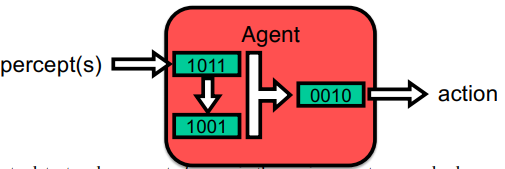
\includegraphics[scale=0.5]{agent_change.png}
\end{center}

\begin{flushleft}
to detect and represent changes in the environment we need rules
\begin{itemize}
  \item whose conditions match against representations of the current and previous precepts 
  \item whose action is to remember (copy) the state representing the current percept for use at the next cycle
\end{itemize}
\end{flushleft}

\subsection{Internal representations}
\begin{itemize}
  \item require more space and incur the cost of maintaining the representation 
  \item allow the choice of actions based on sequences of states, e.g.: to react to change or \textbf{lack of it}
  \item given such internal behaviours, much more complex external behaviours are possible
\end{itemize}

\section{Action selection function}
\begin{itemize}
  \item the action selection function for a reactive agent with state looks like 
  \begin{itemize}
    \item $selectAction : Event × State \rightarrow Action × State$
  \end{itemize}
  \item a reactive agent with state (finite-state machine) can respond to regular sequences of events 
  \item we can add more complex state data structures to increase the capabilities of the agent, e.g.,
  \begin{itemize}
    \item add a stack (pushdown automata) to respond to context-free sequences 
    \item add a random-access array to get a Turing machine, etc.
  \end{itemize}
\end{itemize}

\pagebreak
\section*{Reference section} \label{sec:reference}
\begin{description}
	\item[placeholder] \hfill \\
\end{description}
\end{document}
